The first parameter we measured was the ideal buffer size for random I/O 
on a file. First, let us define what we mean by "ideal buffer size." Since
the time to read data is affected by the amount of data read, we define ideal
buffer size as the size in which we achieve the best throughput (Bytes/s)
with the smallest amount of memory. 

Given the classical formula of Equation~\ref{eq:p1_latency} for the latency 
of a magnetic disk access:

\begin{equation}\label{eq:p1_latency}
Latency = S + R + DataSize/TransferRate + C
\end{equation}

where S = Seek Time, R = Rotational Delay, and C = Controller delay, we 
derive the throughput as $T = \frac{DataSize}{Latency}$. We assume that S, R, 
and C are roughly constant regardless of size, so we represent them as constant K and simplify to Equation~\ref{eq:p1_throughput}:

\begin{equation}\label{eq:p1_throughput}
T = \frac{DataSize}{K + \frac{DataSize}{TransferRate}}
\end{equation}

We expect the throughput to follow the behavior of a rational function
with an asymptote equalling TransferRate as DataSize becomes infinitely large.
Thus, the ideal buffer size is defined as the minimum DataSize for which the 
throughput is equal to the TransferRate. In the virtual machine case, we assume 
that the overhead due to address translation is marginal due to the shadow page 
tables, so we expect the VM throughput to be approximately the same as in the host.

In order to measure the throughput, we used the test described by the pseudocode 
of Figure~\ref{fig:p1code}. We first measured the latency to read a
certain number of bytes from disk. Then we calculated throughput T by dividing 
readSize by the latency. However, there were a few aspects we needed 
to consider in our experiment. Since prefetch occurs on sequential read, 
we avoided the problem of measuring the time to retrieve data from the cache instead
of disk access time by first reading a single byte from the end of the file
and then reading from a random offset, essentially making the Linux readahead
algorithm interpret both reads as random. Moreover, we flushed the cache in
between each change of the readSize. 

\begin{figure}[h!]
\begin{lstlisting}
for readSize := MAX_READ_SIZE to MIN_READ_SIZE do
   clear cache
   open file
   read 1B from the end of the file
   t1 := rdtsc_start()
   read readSize bytes from random offset 
   t2 := rdtsc_end()
   close file
\end{lstlisting} 
\caption{Pseudocode for measuring ideal buffer size}
\label{fig:p1code}
\end{figure}

%% Graphs, Results
\begin{figure}[ht!]
	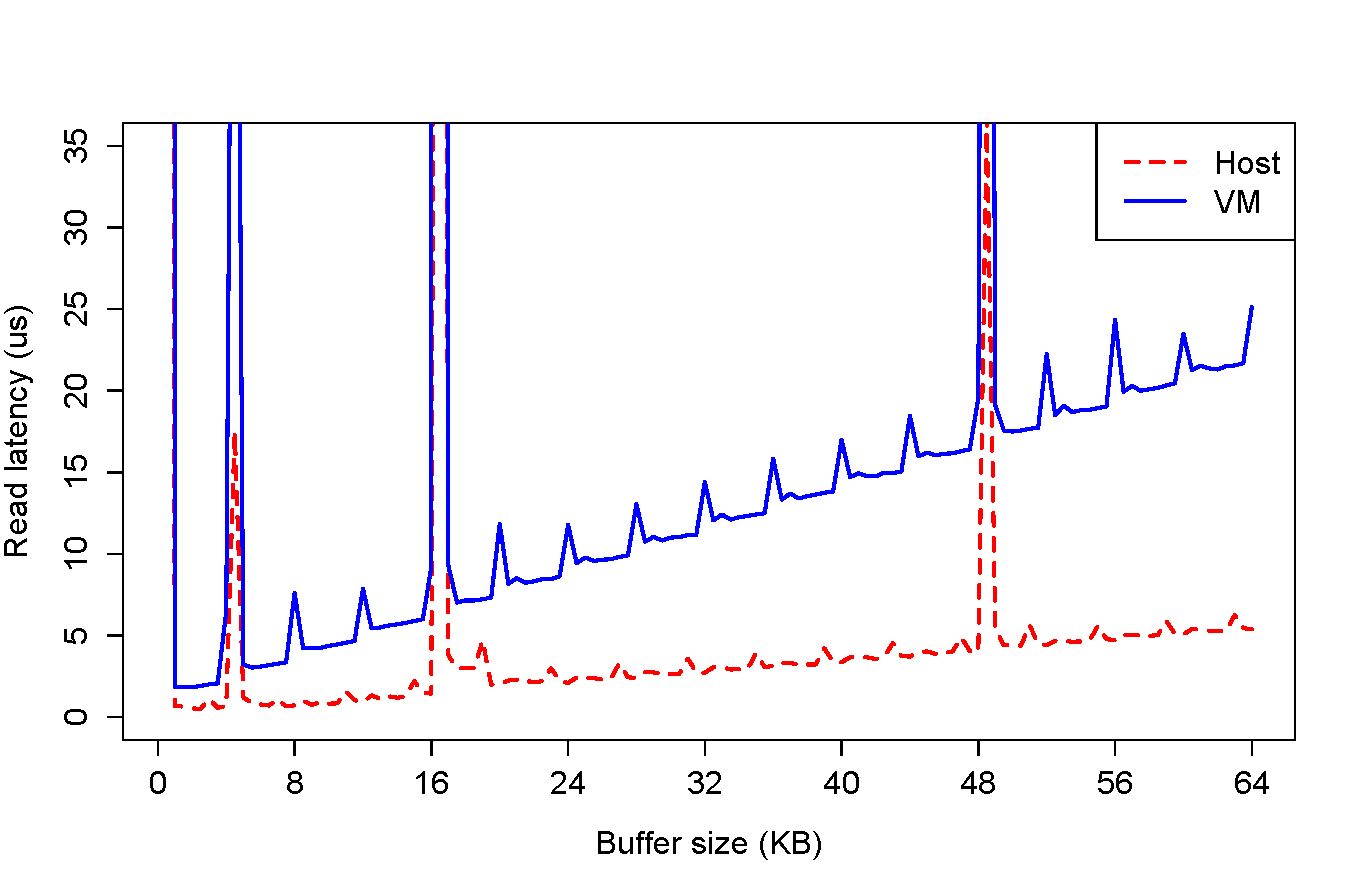
\includegraphics[width=0.5\textwidth]{./figures/p1.pdf}
	\caption{}
	\label{fig:p1graph}
\end{figure}


